\documentclass[11pt,paper=letter]{scrartcl}
\usepackage[wide,noextlink]{cjquines}

\begin{asydef}
  dotfactor = 12;
  defaultpen(0.7);
\end{asydef}

\makeatletter
\def\fps@figure{htbp}
\makeatother

\begin{document}

\title{Hall's marriage theorem}
\author{Carl Joshua Quines}
\date{July 1, 2017}

\maketitle

\begin{abstract}

We define matchings and discuss Hall's marriage theorem. Then we discuss three example problems, followed by a problem set. Basic graph theory knowledge assumed.

\end{abstract}

\section{Matching}

The key to using Hall's marriage theorem is to realize that, in essence, matching things comes up in lots of different ways. The key in thinking about Hall's marriage theorem is to realize that it means, in essence, the obvious matching condition is the only one we need. We'll start by discussing the first, then we'll discuss the second.

What is matching? The canonical example invovles marriage. We have several women who have a list of men they would be happy to marry. Any man would be happy to marry any woman who would be happy to marry him. Is it possible to make all the women happy?

\begin{figure}
  \centering
  \begin{asy}
    draw((0,0)--(1,1), mediumgray);
    draw((0,0)--(0,1), mediumgray);
    draw((1,0)--(2,1), mediumgray);
    draw((2,0)--(0,1), mediumgray);
    draw((3,0)--(0,1), mediumgray);
    draw((3,0)--(1,1), mediumgray);
    draw((3,0)--(3,1), mediumgray);
    draw((0,0)--(3,1), black);
    draw((1,0)--(1,1), black);
    draw((2,0)--(0,1), black);
    draw((3,0)--(2,1), black);
    dot((0,0), black);
    dot((1,0), black);
    dot((2,0), black);
    dot((3,0), black);
    dot((0,1), gray);
    dot((1,1), gray);
    dot((2,1), gray);
    dot((3,1), gray);
  \end{asy}
  \caption{In real life, marriage is \emph{never} as simple as this.}
\end{figure}

We can represent this as a graph, with women as vertices on the top and men as vertices on the bottom. Then we draw edges to show which women like which men. If we look at the darker edges, we see we can pick a bunch of marriages that makes all the women happy.

Such a choice of marriages is called a \emph{matching}. The endpoints of a matching should be different from each other: so no man is married to two or more women and no woman is married to two or more men.

We say that a matching \emph{covers} the set of women if we can make all women happy. A matching that would make all the men happy \emph{covers} the set of men. A matching that makes them all happy covers both sets, and is called a \emph{perfect matching}.

Basically, matching is pairing up two sets to each other. Other natural examples of matching are matching up robots to batteries that fit them, matching companies to people they want to hire, matching kids to gifts they want to receive. In these cases, we can figure out the two sets of vertices and when to draw an edge just fine.

Now, matching things can come up in obvious ways, as above. Sometimes in a problem, we can see that it's asking for a matching, and we can just use Hall's to show a matching exists. But it can come up in non-obvious ways too, where finding the matching is already half of the problem. Take a look at this problem:

\begin{problem*}
  (Kazakhstan 2003) We are given two square sheets of paper with area $2003$. Suppose we divide each of these papers into $2003$ polygons, each of area $1$. (The divisions for the two piece of papers may be distinct.) Then we place the two sheets of paper directly on top of each other. Show that we can place $2003$ pins on the pieces of paper so that all $4006$ polygons have been pierced.
\end{problem*}

\begin{figure}
  \centering
  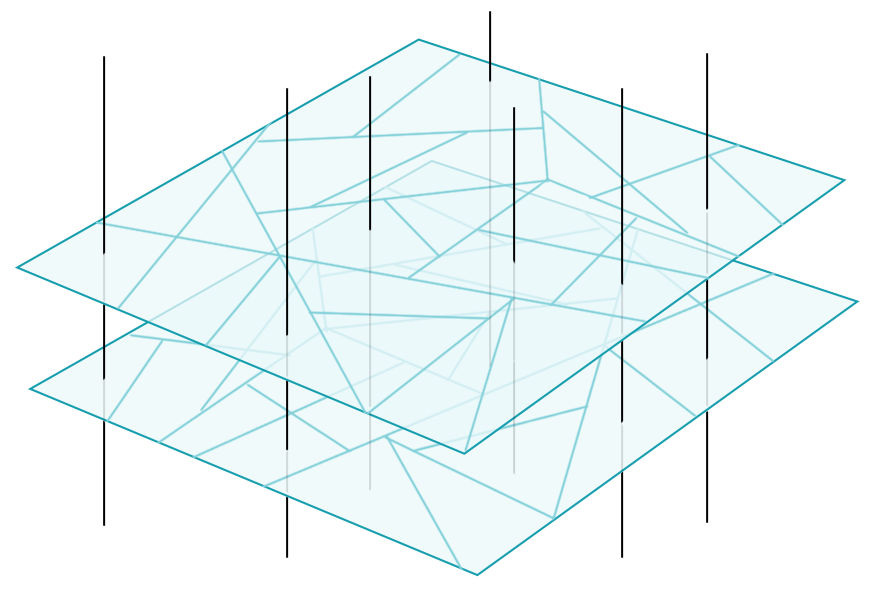
\includegraphics[width=0.75\textwidth]{figure2.png}
  \caption{Utterly mutilating pieces of paper with pins.}
\end{figure}

Where is the matching? There are three questions we need to answer:

\begin{itemize}

\item What are two sets of things we're trying to pair up? In other words, what are the two sets of vertices?

\item When are we allowed to pair up these two things? In other words, when do we draw an edge between two vertices?

\item Are we trying to pair up so that nothing is paired up more than once? In other words, will a matching actually solve the problem?

\end{itemize}

Basically, when we're looking for matchings, we're trying to figure out how to turn a problem into a graph, so we can start matching. \emph{Look at the macro-scale.} How do we turn our polygon problem to a graph?

Let's think about what this question is asking for in the first place. We're looking for pins through the two pieces of paper. A pin pierces one polygon on one sheet and another polygon on the other sheet, so each pin goes through only two polygons. Since we have $2003$ pins and $4006$ polygons, that means all polygons only get pierced by exactly one pin.

\begin{figure}
  \centering
  \begin{asy}
    draw((0,0)--(1,0.2)--(1.4,0.1)--(2,1.1)--(2.1,0.8)--(3.1,0.1), mediumgray);
    draw((0,0.6)--(1,-0.4), mediumgray);
    draw((2,1.1)--(2.1,0.2)--(3.1,0.7), mediumgray);
    draw((3.1,0.7)--(2.7,-0.2)--(2.1,0.8), mediumgray);
    draw((2.7,-0.2)--(3.1,0.7), mediumgray);

    draw((0,0)--(0,0.6), black);
    draw((1,-0.4)--(1,0.2), black);
    draw((1.4,0.1)--(1.4,0.7), black);
    draw((2,0.5)--(2,1.1), black);
    draw((2.1,0.2)--(2.1,0.8), black);
    draw((2.7,-0.2)--(2.7,0.4), black);
    draw((3.1,0.1)--(3.1,0.7), black);

    dot((0,0), lightblue);
    dot((1,-0.4), lightblue);
    dot((1.4,0.1), lightblue);
    dot((2,0.5), lightblue);
    dot((2.1,0.2), lightblue);
    dot((2.7,-0.2), lightblue);
    dot((3.1,0.1), lightblue);

    dot((0,0.6), lightblue);
    dot((1,0.2), lightblue);
    dot((1.4,0.7), lightblue);
    dot((2,1.1), lightblue);
    dot((2.1,0.8), lightblue);
    dot((2.7,0.4), lightblue);
    dot((3.1,0.7), lightblue);
  \end{asy}
  \caption{Looking at the macro-scale. Pins are edges, polygons are vertices.}
\end{figure}

Aha! At this point, we get the idea of the edges of the matching to be the \emph{pins themselves}. A pin pairs one polygon on the first sheet to another polygon on the second sheet, so it's like picking an edge of a graph. That must mean the two sets of things we're trying to pair up are the polygons in the two sheets of paper. We can stick a pin between two polygons if they're directly above each other.

Now we can answer our three matching questions:

\begin{itemize}

\item We're trying to pair up the polygons on one sheet to the polygons on the other sheet.

\item We can pair the polygons only when they're on top of each other. Some part of the first polygon must intersect with some part of the second polygon, so we can place a pin.

\item We're trying to place pins so that each pin hits only two polygons. In other words, if we find a matching of the graph with polygons as vertices and draw edges when they're on top of each other, we're done.

\end{itemize}

At this point, now that we have setup our vertices, our edges, and determined that we're looking for a matching, we're ready to use Hall's to show that a matching exists. But when \emph{does} a matching exist?

\section{Hall's marriage theorem}

Let's go back to our marriage matching. In our previous example, we managed to make everyone happy. But that's not always possible. Consider the graph below:

\begin{figure}
  \centering
  \begin{asy}
    draw((0,1)--(1,0)--(1,1)--(2,0)--(3,1), gray);
    draw((1,0)--(3,1), gray);
    draw((0,0)--(2,1)--(3,0), gray);
    dot((0,0), black);
    dot((1,0), black);
    dot((2,0), black);
    dot((3,0), black);
    dot((0,1), gray);
    dot((1,1), gray);
    dot((2,1), gray);
    dot((3,1), gray);
  \end{asy}
  \caption{There's something wrong here.}
\end{figure}

If you try to find a matching that makes everyone happy, you'll see that you can't. You just can't do it. What's stopping us from doing it? The more we try to find a matching, the more we see what's wrong with this diagram:

\begin{figure}
  \centering
  \begin{asy}
    draw((0,0)--(2,1)--(3,0), mediumgray);
    draw((0,1)--(1,0)--(1,1)--(2,0)--(3,1), black);
    draw((1,0)--(3,1), black);
    dot((0,0), black);
    dot((1,0), black);
    dot((2,0), black);
    dot((3,0), black);
    dot((0,1), gray);
    dot((1,1), gray);
    dot((2,1), gray);
    dot((3,1), gray);
  \end{asy}
  \caption{Even in simplified marriage things can go wrong.}
\end{figure}

This is what's stopping us: these three women. These three women only like two men. But we can't marry the two men to three women. So we can't make everyone happy, because at least one of these women will be sad.

Similarly, if we have two women liking only one man, we can't make everyone happy. If we have four women liking only two men, we can't make everyone happy. If we have $n$ women liking only $m$ men, where $n > m,$ then we can't make everyone happy.

This is called the matching condition. If we pick $n$ women, and they like $m$ men, then we should have $n \leq m.$ Otherwise, if $n > m,$ we can't find a matching. Here's an exercise (which you should do): look at the figure below and confirm that the matching condition holds for any subset of the women.

\begin{figure}
  \centering
  \begin{asy}
    draw((0,0)--(0,1)--(1,0)--(0,1), gray);
    draw((1,0)--(2,1)--(3,0)--(4,1), gray);
    draw((2,0)--(4,1)--(2,0)--(2,1), gray);
    draw((3,0)--(1,1)--(4,0)--(1,1), gray);
    draw((4,0)--(3,1)--(0,0)--(3,1), gray);
    dot((0,0), black);
    dot((1,0), black);
    dot((2,0), black);
    dot((3,0), black);
    dot((4,0), black);
    dot((0,1), gray);
    dot((1,1), gray);
    dot((2,1), gray);
    dot((3,1), gray);
    dot((4,1), gray);
  \end{asy}
  \caption{We can make everyone happy!}
\end{figure}

Now, Hall's says something more than this: if the matching condition is true for all subsets of a set, \emph{then a matching that covers that set exist}. If it doesn't fail the obvious way, then we can make everyone happy. Hall's doesn't tell us anything about finding these matchings, but we can show that a matching exists.

We can write this up in graph theoretical terms. We write $N(W)$ to denote the \emph{neighborhood} of a set $W$: the set of all vertices adjacent to some vertex of $W.$ In our example, our $N(W)$ for a subset $W$ of women would be the set of all men they like. Then this is Hall's:

\begin{theorem*}[Hall's marriage theorem] Let $G$ be a bipartite graph with bipartite sets $X$ and $Y.$ Then there exists a matching that covers $X$ if and only if for each subset $W$ of $X,$ $|W| \leq |N(W)|.$\end{theorem*}

We call the condition, $|W| \leq |N(W)|$ for all subsets $W$ of $X,$ the \emph{matching condition}. If the matching condition holds, a matching exists. We'll abuse terminology: we'll sometimes use \emph{matching condition} to refer only to the inequality $|W| \leq |N(W)|$ itself.

\section{Example problems}

When it's phrased in terms of graphs, Hall's looks quite abstract, but it's actually quite simple. We just have to remember the keys to using Hall's: \emph{matching things comes up in lots of different ways,} and, \emph{the matching condition is the only one we need.} Let's go back to our previous problem.

\begin{problem}
  (Kazakhstan 2003) We are given two square sheets of paper with area $2003.$ Suppose we divide each of these papers into $2003$ polygons, each of area $1.$ (The divisions for the two piece of papers may be distinct.) Then we place the two sheets of paper directly on top of each other. Show that we can place $2003$ pins on the pieces of paper so that all $4006$ polygons have been pierced.
\end{problem}

We already did the first part of the problem earlier, when we found the graph we're looking to find matchings in. We just need to prove that the matching condition holds. To do this, we need to \emph{look at the micro-scale}.

\begin{figure}
  \centering
  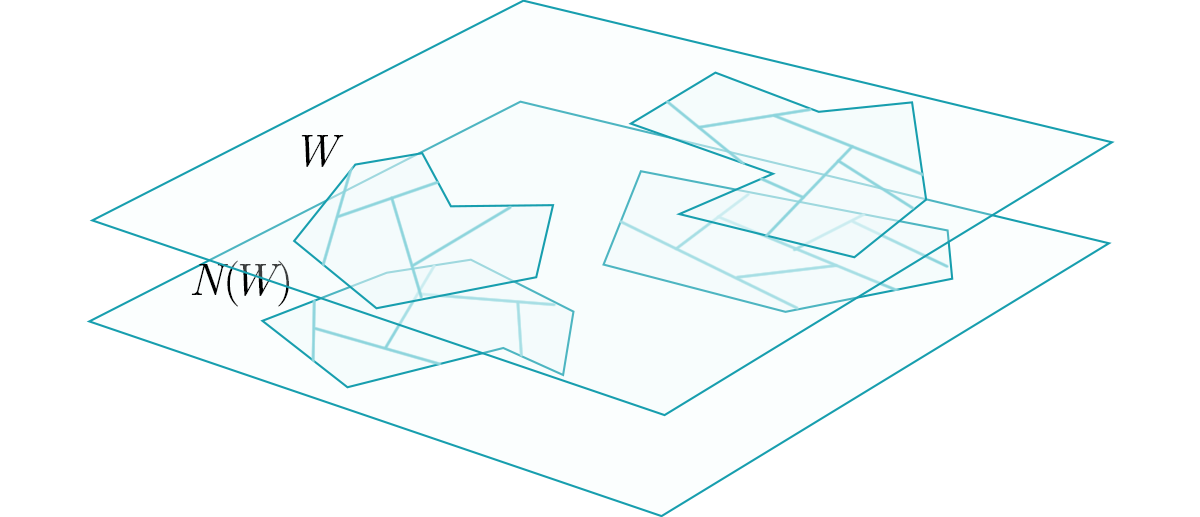
\includegraphics[width=\textwidth]{figure7.png}
  \caption{Looking at the micro-scale to prove the matching condition holds.}
\end{figure}

Suppose that we have such a subset $W$ of the $2003$ polygons on one sheet of paper. We need to prove that there are at least $|W|$ polygons on the other sheet of paper that touch this subset. How do we do this?

We try contradiction. Let's take $W$ and suppose that, say, less than $|W|$ polygons intersect with it on the other sheet. In other words, we have $N(W)$ smaller than $W$. Intuitively, this must mean that the polygons of $W$ are ``smaller'' than those on $N(W),$ because they both occupy the same area\dots

Area. Aha! That's the one piece of information we haven't used yet, the fact that the polygons have area $1$. The polygons of $W$ have an area of exactly $|W|,$ and the polygons of $N(W)$ have an area of exactly $|N(W)|.$ But the region $N(W)$ has to contain the region of $W$ entirely, so that means we have $|W| \leq |N(W)|.$ This is the matching condition -- and remember, \emph{the matching condition is the only one we need}. Let's write this up nicely:

\begin{figure}
  \centering
  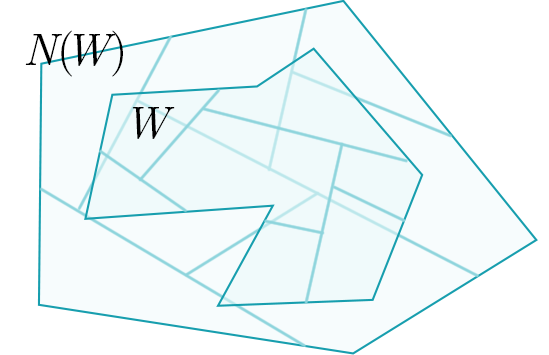
\includegraphics[width=0.5\textwidth]{figure8.png}
  \caption{$N(W)$ has to contain $W$ entirely.}
\end{figure}

\begin{proof}
  Consider the bipartite graph with the bipartite sets being the $2003$ polygons in either sheet of paper. Connect two vertices from both bipartite sets if and only if their polygons have a non-empty intersection when placed on top of each other.

  Consider a subset $W$ of one of these bipartite sets. This subset has area $|W|,$ as all polygons have area $1.$ Its neighbor set $N(W)$ has area $|N(W)|.$ However, note that the region bounded by $W$ is only a subset of the region bounded by $N(W).$

  Thus $|W| \leq |N(W)$ for any subset $W,$ and by Hall's marriage theorem there exists a matching from one set of polygons to the other. We use this matching to find appropriate positions for the pins.
\end{proof}

From this problem we have two main ideas:

\begin{itemize}

\item Look at the macro-scale: to find the matching, we ask ourselves the three matching questions. What are the two sets of things we're trying to pair up? When are we allowed to pair up these two things? Are we trying to pair up so that nothing is paired up more than once?

\item Look at the micro-scale: to prove the matching condition, we consider a subset and its neighbor set. Usually these two sets are close to each other in some way, so we need to look at local, small stuff rather than global, large stuff.

\end{itemize}

The next problem we'll try is one that also doesn't have an obvious matching!

\begin{problem}
  (AMSP C3 2014) Let $n \in \{1, 2, \ldots, 8\}.$ Consider an $8 \times 8$ chessboard with the property that on each column and each row there are exactly $n$ pieces. Prove that we can choose $8$ pieces such that no two of them are in the same row or same column.
\end{problem}

\begin{figure}
  \centering
  \begin{asy}
    size(4cm);
    dotfactor = 8;
    for (real i = 0; i <= 8; ++i) {
      draw((i-0.5, -0.5)--(i-0.5, 7.5));
      draw((-0.5, i-0.5)--(7.5, i-0.5));
    }
    dot((0,0), gray);
    dot((1,4), gray);
    dot((2,3), gray);
    dot((3,1), gray);
    dot((4,5), gray);
    dot((5,7), gray);
    dot((6,6), gray);
    dot((7,2), gray);
    dot((0,1), gray);
    dot((0,4), gray);
    dot((1,0), gray);
    dot((1,6), gray);
    dot((2,2), gray);
    dot((2,7), gray);
    dot((3,3), gray);
    dot((3,6), gray);
    dot((4,1), gray);
    dot((4,3), gray);
    dot((5,0), gray);
    dot((5,4), gray);
    dot((6,2), gray);
    dot((6,5), gray);
    dot((7,5), gray);
    dot((7,7), gray);
  \end{asy}
  \caption{A case when $n = 3$.}
\end{figure}

What is our tip-off for Hall's? To be honest, looking for Hall's tip-offs is pretty hard. So let's pretend we didn't see this problem in a handout for Hall's marriage theorem and try to solve it.

A good idea, as always, is to \emph{look at the macro-scale.} What are we looking for in this problem? We're looking for $8$ pieces so that no two of them are in the same row or same column. What does this look like? It looks kinda like this:

\begin{figure}
  \centering
  \begin{asy}
    size(5cm);
    dotfactor = 8;
    for (real i = 0; i <= 8; ++i) {
      draw((i-0.5, -0.5)--(i-0.5, 7.5));
      draw((-0.5, i-0.5)--(7.5, i-0.5));
    }
    dot((0,0), black);
    dot((1,4), black);
    dot((2,3), black);
    dot((3,1), black);
    dot((4,5), black);
    dot((5,7), black);
    dot((6,6), black);
    dot((7,2), black);
    dot((0,1), mediumgray);
    dot((0,4), mediumgray);
    dot((1,0), mediumgray);
    dot((1,6), mediumgray);
    dot((2,2), mediumgray);
    dot((2,7), mediumgray);
    dot((3,3), mediumgray);
    dot((3,6), mediumgray);
    dot((4,1), mediumgray);
    dot((4,3), mediumgray);
    dot((5,0), mediumgray);
    dot((5,4), mediumgray);
    dot((6,2), mediumgray);
    dot((6,5), mediumgray);
    dot((7,5), mediumgray);
    dot((7,7), mediumgray);
  \end{asy}
  \caption{Solving the above example.}
\end{figure}

No two are in the same row or same column means that each row and each column has exactly one selected piece on it. Also, there's a natural bijection between the rows and columns: since each row and each column has exactly one selected piece, map the row to the column containing that row's selected piece. (In general, if we have two sets with the same number of elements, it's a good idea to try and look for a bijection.)

So we're trying to construct a bijection between the rows and columns, one that uses the pieces to connect a row to its corresponding column. Hey! \emph{This} is our tip-off for Hall's. Selecting $8$ pieces is the same as selecting $8$ rows and $8$ corresponding columns! We're \emph{matching rows to columns} using the pieces to decide which matchings are allowed. Let's make it more specific by answering our three matching questions:

\begin{itemize}

\item \emph{What are two sets of things we're trying to pair up?} We're trying to pair up rows with columns.

\item \emph{When are we allowed to pair up these two things?} We can only pair rows and columns that have a piece in their intersection.

\item \emph{Are we trying to pair up so that nothing is paired up more than once?} We only want to select one piece per row and column, so we're trying to pair up such that no row or no column is paired up more than once. A matching from rows to columns will solve the problem.

\end{itemize}

Now that we have a matching we want to show exists, let's try to prove the matching condition. Once again, we \emph{look at the micro-scale:} consider a subset $W$ of the rows and prove that its neighbor set $N(W)$ is larger than it.

Let's think about this. Each row in $W$ will have $n$ pieces on it. That means each row in $W$ is connected to exactly $n$ columns in $N(W)$. For the same reason, each column in $N(W)$ is connected to at most $n$ rows in $W$. (It can be less than $n,$ because not all of the pieces on that column might lie on the rows of $W$. But it can't be more.)

\begin{figure}
  \centering
  \begin{asy}
    size(5cm);
    dotfactor = 8;
    filldraw((-0.5,-0.5)--(7.5,-0.5)--(7.5,1.5)--(-0.5,1.5)--cycle, lightgray, white);
    filldraw((-0.5,3.5)--(7.5,3.5)--(7.5,4.5)--(-0.5,4.5)--cycle, lightgray, white);
    filldraw((-0.5,-0.5)--(1.5,-0.5)--(1.5,7.5)--(-0.5,7.5)--cycle, lightgray, white);
    filldraw((2.5,-0.5)--(5.5,-0.5)--(5.5,7.5)--(2.5,7.5)--cycle, lightgray, white);
    for (real i = 0; i <= 8; ++i) {
      draw((i-0.5, -0.5)--(i-0.5, 7.5));
      draw((-0.5, i-0.5)--(7.5, i-0.5));
    }
    dot((0,0), gray);
    dot((1,4), gray);
    dot((2,3), gray);
    dot((3,1), gray);
    dot((4,5), gray);
    dot((5,7), gray);
    dot((6,6), gray);
    dot((7,2), gray);
    dot((0,1), gray);
    dot((0,4), gray);
    dot((1,0), gray);
    dot((1,6), gray);
    dot((2,2), gray);
    dot((2,7), gray);
    dot((3,3), gray);
    dot((3,6), gray);
    dot((4,1), gray);
    dot((4,3), gray);
    dot((5,0), gray);
    dot((5,4), gray);
    dot((6,2), gray);
    dot((6,5), gray);
    dot((7,5), gray);
    dot((7,7), gray);
  \end{asy}
  \caption{Here, $W$ contains the fourth, seventh, and eighth rows from the top.}
\end{figure}

This gives us the idea to start \emph{counting the degree} of each set. There are $|W|$ rows in $W,$ with a total of $n|W|$ edges coming out of it, as each row has $n$ edges coming out of it. These connect to $N(W).$ But $N(W)$ has at most $n|N(W)|$ edges coming out of it. Thus we have $n|W| \leq n|N(W)|\ldots$ and this is the matching condition. We are done.

\begin{proof}
  Consider the bipartite graphs with the bipartite sets being the rows and columns. Connect two vertices from both bipartite sets if and only if their row and column intersects in a square with a piece on it.

  Consider a subset $W$ of the rows. Each row has $n$ pieces on it, and is thus connected to $n$ columns. Thus there are $n|W|$ edges from $W$ to $N(W).$ Since each column has $n$ pieces on it, each column in $N(W)$ has at most $n$ edges to $W.$ Thus there are at most $n|N(W)|$ edges from $N(W)$ to $W.$

  From this we have $n|W| \leq n|N(W)|,$ for any subset $W,$ and by Hall's marriage theorem there exists a matching from the rows to the columns. This matches each row to exactly one column, and the intersections of each row and each column determines a piece. These $8$ determined pieces are a selection such that no two are in the same row or same column.
\end{proof}

We gain two new ideas in using Hall's marriage theorem:

\begin{itemize}

\item If we have a table and we're trying to match rows to columns such that no two rows match to one column or vise-versa, then Hall's on the rows and columns might help. Then we draw an edge between two vertices if their row and column intersects in a square with a certain property.

\item In trying to prove the matching condition, we can try examining the degree of each vertex in the subset and each vertex in the neighbor set. Remember that a subset and its neighbor set have the same number of edges connecting them.

\end{itemize}

Finally we try a problem from the Canada MO.

\begin{problem}
  (Canada 2006/3 \cite{canada}) In a rectangular array of nonnegative reals with $m$ rows and $n$ columns, each row and each column contains at least one positive element. Moreover, if a row and a column intersect in a positive element, then the sums of their elements are the same. Prove that $m = n$.
\end{problem}

\begin{figure}
  \centering
  \begin{asy}
    size(4.5cm);
    for (real i = 0; i <= 6; ++i) {
      draw((i-0.5, -0.5)--(i-0.5, 5.5));
      draw((-0.5, i-0.5)--(5.5, i-0.5));
    }

    label("0", (0, 0), mediumgray);
    label("1", (1, 0));
    label("0", (2, 0), mediumgray);
    label("0", (3, 0), mediumgray);
    label("0", (4, 0), mediumgray);
    label("2", (5, 0));

    label("0", (0, 1), mediumgray);
    label("0", (1, 1), mediumgray);
    label("1", (2, 1));
    label("0", (3, 1), mediumgray);
    label("1", (4, 1));
    label("0", (5, 1));

    label("4", (0, 2));
    label("0", (1, 2), mediumgray);
    label("0", (2, 2), mediumgray);
    label("0", (3, 2), mediumgray);
    label("0", (4, 2), mediumgray);
    label("0", (5, 2), mediumgray);

    label("0", (0, 3), mediumgray);
    label("0", (1, 3), mediumgray);
    label("0", (2, 3), mediumgray);
    label("5", (3, 3));
    label("0", (4, 3), mediumgray);
    label("0", (5, 3), mediumgray);

    label("0", (0, 4), mediumgray);
    label("2", (1, 4));
    label("0", (2, 4), mediumgray);
    label("0", (3, 4), mediumgray);
    label("0", (4, 4), mediumgray);
    label("1", (5, 4));

    label("0", (0, 5), mediumgray);
    label("0", (1, 5), mediumgray);
    label("1", (2, 5));
    label("0", (3, 5), mediumgray);
    label("1", (4, 5));
    label("0", (5, 5), mediumgray);
  \end{asy}
  \caption{A $6 \times 6$ array that satisfies the conditions.}
\end{figure}

There are ways to solve this problem without Hall's, but we will follow the thought process of a solution that does. Now let's pretend we didn't see this in a Hall's handout.

Each row and each column contains at least one positive element. We observe that rows and columns that intersect in a positive element are related in some way. Observe that if a row intersects with two columns, then both columns have the same sum -- that means that there has to be some kind of connection between rows and columns. Intuitively, there will be lots of rows and columns with the same sum.

This is when we realize to treat rows and columns as separate entities: as individual parts of the array. We can then examine the connection between rows and columns, and we recognize that the problem can be recast in graph theory: our vertices are rows and columns, and we draw an edge if they intersect at a positive element, producing a bipartite graph.

The moment we recognize the bipartite graph, we realize that Hall's can help. We can try to show a matching exists. There's no reason to favor one set over the other: we only need to show a matching covers the rows, showing $m \leq n$. By symmetry, the same argument applies for the columns, so $m \geq n$. This implies $m = n$. This is, in fact, the main idea: we've looked at the macro-scale and we've realized the problem as a graph matching one.

We need to prove that for every set $W$ of rows, $|W| \leq |N(W)|$. This seems quite hard to do directly, since we have to do it for \emph{every} set of rows. The only condition we have is that rows and columns that are adjacent in the graph have the same sum. In this case, we try to prove the matching condition by contradiction, which is an important strategy: \emph{try contradiction}.

\begin{figure}
  \centering
  \begin{asy}
    size(4.5cm);
    filldraw((-0.5,-0.5)--(5.5,-0.5)--(5.5,1.5)--(-0.5,1.5)--cycle, lightgray, white);
    filldraw((-0.5,3.5)--(5.5,3.5)--(5.5,4.5)--(-0.5,4.5)--cycle, lightgray, white);
    filldraw((1.5,-0.5)--(2.5,-0.5)--(2.5,5.5)--(1.5,5.5)--cycle, lightgray, white);
    filldraw((3.5,-0.5)--(4.5,-0.5)--(4.5,5.5)--(3.5,5.5)--cycle, lightgray, white);
    for (real i = 0; i <= 6; ++i) {
      draw((i-0.5, -0.5)--(i-0.5, 5.5));
      draw((-0.5, i-0.5)--(5.5, i-0.5));
    }
    label("+", (2, 4));
    label("+", (4, 4));
    label("+", (2, 1));
    label("+", (4, 0));
  \end{asy}
  \caption{A set of rows matching less columns. Here, $+$ is a positive entry.}
\end{figure}

Assume there exists some set $W$ of rows such that $|W| > |N(W)|$. Now we can try to use the row and column sums to get a contradiction. We see that none of the entries in the rows of $W$ outside of the columns are positive, because otherwise they'd be in $N(W)$. So we simplify: the row sums of $W$ are restricted to the intersections with the columns of $N(W)$.

Now we remember the condition. Each column in $N(W)$ has the same sum of some row in $W$. Aha! Since each column has the same sum of some row, and there are more rows than columns, the column sums should be a proper subset of the row sums. But the column-sum should be at least the row-sum, as all the other elements in the column are nonnegative!

More specifically, if the row sums are $w_1, w_2, \ldots, w_{|W|}$, the row-sum will be the sum of all of them. Each column matches to one $w_i$, so the column sums are a subset of the row sums. The sum of the positive elements in the rows is simply the sum of all the $w_i$. Since all the positive elements in the rows lie in the columns, the column-sum should be at least the sum of all the $w_i$. This is the contradiction, since the column sums are a subset of the row sums.

\begin{figure}
  \centering
  \begin{asy}
    size(4.5cm);
    filldraw((-0.5,3.5)--(5.5,3.5)--(5.5,4.5)--(-0.5,4.5)--cycle, lightgray, white);
    filldraw((1.5,-0.5)--(2.5,-0.5)--(2.5,5.5)--(1.5,5.5)--cycle, lightgray, white);
    filldraw((3.5,-0.5)--(4.5,-0.5)--(4.5,5.5)--(3.5,5.5)--cycle, lightgray, white);
    for (real i = 0; i <= 6; ++i) {
      draw((i-0.5, -0.5)--(i-0.5, 5.5));
      draw((-0.5, i-0.5)--(5.5, i-0.5));
    }
    label("+", (2, 4));
    label("+", (4, 4));
  \end{asy}
  \caption{What if the same row matches to two columns?.}
\end{figure}

Are we done? Not quite yet: what if the same row matches to two columns? Then our argument would be moot. This is when we realize we haven't used the ``at least one positive element in each row'' condition: since each row has at least one positive element, each row should be adjacent to at least one column.

Thus if $|W|$ rows are adjacent to less columns, some two rows would be adjacent to the same column. If a row is adjacent to two columns, then some other row would have to be adjacent to one of those columns, otherwise we wouldn't have $|W| > |N(W)|$. So the column sums really are a subset: we can pick one $w_i$ for each column, without repeating any. This finishes the proof.

\begin{proof}
  Consider the bipartite graph with vertex sets as rows and columns. Two vertices are adajcent if and only if their row and column intersect at a positive element. 

  Assume there exists some subset $W$ of the rows such that $|W| > |N(W)|$. Since each row and column has at least one positive element, it must be the case that the degree of each row in $W$ is at least one, therefore it is the case each vertex in $N(W)$ is adjacent to at least one vertex in $W$.

  Thus to each column in $N(W)$ we can associate one adjacent vertex in $W$ without repeating any of $W$'s vertices. It must follow that the sum of the entries in $N(W)$ is less than the sum of the entries in $W$. However, since the rows of $W$ contain no positive elements outside of their intersections with $N(W)$, the sum of the entries in $W$ is at most the sum of the entries in $N(W)$.

  This is a contradiction. Thus for all subset $W$ of the rows we have $|W| \leq |N(W)|$. Applying Hall's shows that a matching exists that covers the rows, therefore $m \leq n$. By symmetry, a matching exists that covers the columns as well, therefore $m \geq n$. Therefore $m = n$.
\end{proof}

We finish up our idea list with one new insight:

\begin{itemize}
  \item In proving the matching condition, if you don't see an easy way to apply the conditions given in the problem, try contradiction: assume some subset doesn't satisfy the matching condition, and try to show this leads to a contradiction.
\end{itemize}

\section{Summary}

Here's the list of heuristics we found when solving the example problems:

\begin{itemize}

\item Hall's marriage theorem can come up in expected and unexpected ways. The key is to look for two sets which we want to match with one another: finding these sets is often half of the problem. The other half is proving that the matching condition holds.

\item Look at the macro-scale: to find the matching, we ask ourselves the three matching questions. What are the two sets of things we're trying to pair up? When are we allowed to pair up these two things? Are we trying to pair up so that nothing is paired up more than once?

\item Look at the micro-scale: to prove the matching condition, we consider a subset and its neighbor set. Usually these two sets are close to each other in some way, so we need to look at local, small stuff rather than global, large stuff.

\item If we have a table and we're trying to match rows to columns such that no two rows match to one column or vise-versa, then Hall's on the rows and columns might help. Then we draw an edge between two vertices if their row and column intersects in a square with a certain property.

\item In trying to prove the matching condition, we can try examining the degree of each vertex in the subset and each vertex in the neighbor set. Remember that a subset and its neighbor set have the same number of edges connecting them.

\item In proving the matching condition, if you don't see an easy way to apply the conditions given in the problem, try contradiction: assume some subset doesn't satisfy the matching condition, and try to show this leads to a contradiction.

\item For the harder problems in this set, using Hall's theorem will probably not be the main idea in the proof, but rather only used as an intermediate step in the solution. These are a combinatorics problems, with a lot of freedom: try plenty of things!

\end{itemize}

\section{Problems}

While some of the problems can be solved without Hall's, the hints assume use of Hall's theorem. Straightforward problems usually involve a clear application with a clear proof of the matching condition, involved problems require a bit more ingenuity, while challenging problems are difficult enough to be olympiad problems. Problems are very roughly sorted by difficulty.

\subsection{Straightforward}

\begin{enumerate}

\item (Combinatorial Hall's) Let $S_1, S_2, \ldots, S_m$ be sets. A transversal is an ordered set $(s_1, s_2, \ldots, s_m)$ such that each of the $s_i$'s are different and $s_i \in S_i$. Prove that there exists a transversal if and only if the union of any $k$ sets has at least $k$ elements.

\item (K\"onig's Marriage Theorem) Prove that if all the vertices of a bipartite graph have the same degree, then it has a perfect matching.

\item (Bollob\'as \cite{bollobas}) A bipartite graph $G$ has vertex sets $X$ and $Y$. Let $A$ be the set of vertices of $G$ with the largest degree. Prove there exists a matching that covers $A \cap X$. Why does this imply the above problem?

\item We have a regular deck of $52$ playing cards, with exactly $4$ cards of each of the $13$ ranks. The cards have been randomly dealt into $13$ piles, each with $4$ cards in it. Prove that there is a way to take a card from each pile so that after we take a card from every pile, we have exactly a card of every rank.

Prove that, in fact, we can go further: after taking a card of every rank, there are $3$ cards left in each pile. We can then take a card of every rank once more, leaving $2$ cards in each pile. Finally, we do it once more, and the remaining card in each pile must be of every rank.

\item (Putnam 2012/B3 \cite{putnam}) Suppose $2m$ teams play in a round-robin tournament. Over a period of $2m-1$ days, every team plays every other team exactly once. There are no ties. Show that for each day we can select a winning team, without selecting the same team twice.

\item A class of $100$ is participating in an oral exam. The committee consists of $25$ members. Each student is interviewed by one member of the committee. It is known that each student likes at least $10$ committee members. Prove that we can arrange the exam schedule such that each student is interviewed by one of the committee members that he likes, and each committee member interviews at most $10$ students.

\end{enumerate}

\subsection{Involved}

\begin{enumerate}

\item Let $G$ be a connected bipartite graph with bipartite sets $X$ and $Y$. Suppose that for any two adjacent vertices $x \in X$ and $y \in Y$, we have $\deg(x) \geq \deg(y)$. Prove that $G$ has a matching that covers $X$.

\item (Making Latin squares) We are given an $n \times k$ board with $k < n$ such that in every square there is a number from $1$ to $n$. We know that in every column and every row no number repeats itself. Show that we can extend this to an $n \times n$ board with a number from $1$ to $n$ in each square, such that in every row and every column no number repeats itself.

\item (Baltic Way 2013/6 \cite{baltic}) Santa Claus has at least $n$ gifts for $n$ children. For $i\in\{1,2, ... , n\}$, the $i$th child considers $x_i > 0$ of these items to be desirable. Assume that $$\dfrac{1}{x_1}+\cdots+\dfrac{1}{x_n}\le1.$$ Prove that Santa Claus can give each child a gift that this child likes. 

\item (Bollob\'as \cite{bollobas}) All the vertices of a bipartite graph have the same degree $d$. What is the maximum number of edges we can remove to ensure the resulting graph has a perfect matching?

\item (IMC 2011/2/2b \cite{imc}) An alien race has three genders: male, female and emale. A \emph{married triple} consists of three persons, one from each gender, who all like each other. Any person is allowed to belong to at most one married triple. A special feature of this race is that feelings are always mutual -- if $x$ likes $y$, then $y$ likes $x$.

The race is sending an expedition to colonize a planet. The expedition has $n$ males, $n$ females, and $n$ emales. It is known that every expedition member likes at least $k$ persons of each of the two other genders. The problem is to create as many married triples as possible to produce healthy offspring so the colony could grow and prosper.

Show that if $k \geq 3n/4$, then it is always possible to create $n$ disjoint married triples, thus marrying all of the expedition members.

\item (K\"onig's Theorem) An $m \times n$ table is filled with $0$s and $1$s. Call a column or a row a \emph{line}. Prove that the minimal number of lines containing all the $1$s of $A$ is precisely the maximal number of $1$s with no two in the same line.

\end{enumerate}

\subsection{Challenging}

\begin{enumerate}

\item (AMSP C3 2014 \cite{amsp}) An $n \times n$ table is filled with $0$ and $1$ so that if we choose any $n$ cells, no two of them on the same row or column, then at least one contains $1$. Prove that we can find $i$ rows and $j$ columns so that $i + j \geq n + 1$ and their intersection contains only $1$s. 

\item (Vietnam TST 2001/3 \cite{vietnam}) A club has $42$ members. Suppose that for any $31$ members in this club, there exists a boy and a girl among these $31$ members who know each other. Show that we can form $12$ disjoint pairs of people, each pair having one boy and one girl, such that the people in each pair know each other.

\item (ISL 2010/C2 \cite{islc2}) On some planet, there are $2^N$ countries, where $N\ge4$. Each country has a flag $N$ units wide and one unit high composed of $N$ fields of size $1 \times 1,$ each field being either yellow or blue. No two countries have the same flag.

We say that a set of $N$ flags is diverse if these flags can be arranged into an $N \times N$ square so that all $N$ fields on its main diagonal will have the same color. Determine the smallest positive integer $M$ such that among any $M$ distinct flags, there exist $N$ flags forming a diverse set.

\item (WOOT 2011) A table has $m$ rows and $n$ columns with $m, n > 1$. The following permutations of its $mn$ elements are permitted: any permutation leaving each element in the same row (a ``horizontal move''), and any permutation leaving each element in the same column (a ``vertical move''). Find the smallest integer $k$ such that any permutation of the $mn$ elements can be realized by at most $k$ permitted moves.

\item (ISL 2012/C5 \cite{islc5}) The columns and the rows of a $3n \times 3n$ square board are numbered $1,2,...,3n$. Every square $(x,y)$ with $1 \leq x,y \leq 3n$ is colored asparagus, byzantium or citrine according as the modulo $3$ remainder of $x+y$ is $0, 1$ or $2$ respectively. One token colored asparagus, byzantium or citrine is placed on each square, so that there are $3n^2$ tokens of each color.

Suppose that one can permute the tokens so that each token is moved to a distance of at most $d$ from its original position, each asparagus token replaces a byzantium token, each byzantium token replaces a citrine token, and each citrine token replaces an asparagus token. Prove that it is possible to permute the tokens so that each token is moved to a distance of at most $d + 2$ from its original position, and each square contains a token with the same color as the square.

\item (ISL 2006/C6 \cite{islc6}) A holey triangle is an upward equilateral triangle of side length $n$ with $n$ upward unit triangular holes cut out. A diamond is a $60^\circ-120^\circ$ unit rhombus. Prove that a holey triangle $T$ can be tiled with diamonds if and only if the following condition holds: Every upward equilateral triangle of side length $k$ in $T$ contains at most $k$ holes, for $1\leq k\leq n$.

\end{enumerate}

\newpage

\section{Hints}

\subsection{Straightforward}

\begin{enumerate}

\item Let the elements of $X$ be the sets and the elements of $Y$ be the elements of the union of all the sets.

\item First show $X$ and $Y$ have the same number of vertices.

\item Try contradiction. Count the degrees of the vertices.

\item The sets are the thirteen ranks and the thirteen piles.

\item The sets are the $2m$ teams and the $2m-1$ days. Try contradiction.

\item Instead of $25$ commitee members, consider each member having $10$ ``time slots'', to account for the fact each member interviews at most $10$ students.

\end{enumerate}

\subsection{Involved}

\begin{enumerate}

\item How can we use $\deg(x) \geq \deg(y)$ to prove the matching condition?

\item Use induction: create $n \times (k + 1)$ from $n \times k$. Try $k = n-1$ case and generalize.

\item The obvious choice of sets works; prove the matching condition by contradiction.

\item The answer is $d-1$. Why won't deleting edges break the matching condition?

\item First marry males to females, then marry the male-female pairs to emales.

\item The sets are rows and columns. Choose vertices adjacent to all edges, show by Hall's some matching covers these vertices.

\end{enumerate}

\subsection{Challenging}

\begin{enumerate}

\item The sets are rows and columns. Prove the contrapositive.

\item Try contradiction. Use the condition to force adjacent vertices.

\item The answer is $M = 2^{N-2} + 1$. To prove the upper bound, construct two graphs with the rows and columns as bipartite sets: one graph has an edge if the square is yellow, the other has an edge if the square is blue.

\item We only need three moves. Get all the pieces in their proper rows in two moves.

\item Without loss of generality, we only need to prove that the $A$-tokens can be moved to distinct $A$-squares that have distance at most $d+2$ from their original places. Match tokens to squares.

\item We're matching downward unit triangles to adjacent upward unit triangles. For necessity, consider largest set of downward triangles that break condition. These triangles can't be disjoint, use this to construct contradiction.

\end{enumerate}

\begin{thebibliography}{99}

\bibitem{canada} \url{http://aops.com/community/c6h130634}

\bibitem{bollobas} B\'ela Bollob\'as, \emph{Modern Graph Theory}.

\bibitem{putnam} \url{http://kskedlaya.org/putnam-archive/2012s.pdf}

\bibitem{baltic} \url{http://aops.com/community/c6h569075}

\bibitem{imc} \url{http://imc-math.org.uk/imc2011/imc2011-day2-solutions.pdf}

\bibitem{amsp} \url{http://aops.com/community/c6h1154372}

\bibitem{vietnam} \url{http://aops.com/community/c6h42400}

\bibitem{islc2} \url{http://aops.com/community/c6h418686}

\bibitem{islc5} \url{http://aops.com/community/c6h546172}

\bibitem{islc6} \url{http://aops.com/community/c6h155700}

\end{thebibliography}

If anyone knows the sources to any problem without one, see an error, have a correction, or have a question, please do not hestitate to contact me at \mailto{cj@cjquines.com}.

\end{document}
